\documentclass[11pt,compress]{beamer}

\RequirePackage[francais]{babel}
\RequirePackage{amsfonts,amssymb,amsmath,mathtools}
\RequirePackage[utf8]{inputenc}
\RequirePackage[T1]{fontenc}
\RequirePackage{lmodern}
\RequirePackage{mathpazo}
\usepackage{tikz}

\definecolor{LHCblue}{RGB}{10, 73, 132}
\usecolortheme[named=LHCblue]{structure}
\usepackage[bars]{beamerthemetree} %Beamer theme v 2.2
\usefonttheme[onlymath]{serif}
%\usepackage{kerkis}
\setbeamercovered{highly dynamic}
\usetheme{Ilmenau} % Beamer theme v 3.0
\useoutertheme[subsection=true]{smoothbars}%Beamer Outer Theme-circles on top
\usefonttheme{serif}
\useinnertheme{circles} %rectangle bullet points instead of circle ones
\usepackage{beamerthemebars}

\setbeamerfont{section in toc}{size=\small}
\setbeamerfont{subsection in toc}{size=\small}
\setbeamercolor{subsection in toc}{fg=LHCblue!40!black}
\expandafter\def\expandafter\insertshorttitle\expandafter{%
  \insertshorttitle\hfill%
  \insertframenumber\,/\,\inserttotalframenumber}
\setbeamertemplate{navigation symbols}{}%remove navigation symbols

\AtBeginSection[]
{
  \begin{frame}
  \frametitle{Plan}
  \begin{columns}[t]
  \begin{column}{5cm}
  \tableofcontents[sections={1-3},currentsection, hideothersubsections]
  \end{column}
  \begin{column}{5cm}
  \tableofcontents[sections={4-6},currentsection,hideothersubsections]
  \end{column}
  \end{columns}
  \end{frame}
}

\author{Clément PARISOT}
\title{Young engineers seminar}
\subtitle{Grid'5000 support and services orchestration}
\institute{IJD INRIA Nancy\\MADYNES Team\vspace{2.75cm}}
\begin{document}
\titlegraphic{%
\begin{center}

\includegraphics[height=1.25cm]{figures/inria-logo}
\hspace{30mm}

\includegraphics[height=1.25cm]{figures/g5k-logo}
\end{center}
}
\date{\scriptsize 2016/11/09}

{
\setbeamertemplate{footline}{} 
\setbeamertemplate{headline}{}
\usebackgroundtemplate{
  \begin{tikzpicture}
    \path [outer color = LHCblue!15, inner color = white]
      (0,0) rectangle (\paperwidth,\paperheight);
  \end{tikzpicture}}
\begin{frame}[plain]
  \titlepage
\end{frame}
}
\addtocounter{framenumber}{-1}
\institute{IJD INRIA Nancy}

\begin{frame}
\frametitle{Summary}
\begin{columns}[t]
  \begin{column}{5cm}
  \tableofcontents[sections={1-3},hideothersubsections]
  \end{column}
  \begin{column}{5cm}
  \tableofcontents[sections={4-6},hideothersubsections]
  \end{column}
  \end{columns}
\end{frame}

\section{Introduction}
\subsection{Grid'5000}
\begin{frame}
\frametitle{Grid'5000 platform}
\begin{block}{}
\textbf{Grid'5000}: a large-scale and versatile distributed testbed for experiments-driven research on parallel and distributed systems
\end{block}
\begin{itemize}
\item Created in 2003
\item Need of a bigger and efficient platform for experiments

\item Give users root access to the compute nodes
\item Deploy environment
\item Allows experiments on all the software layers
\end{itemize}
\end{frame}

\begin{frame}
\frametitle{Grid'5000 today (2016/11)}
\begin{columns}[c]
  \begin{column}{6cm}
	\begin{itemize}
	\item 7 sites in France
	\item 1 site in Luxembourg
	\item 10G dedicated Renater network
	\item 30 clusters
	\item 903 nodes
	\item 8700 cores
	\item 84 accelerators (Xeon Phi/GPU)
	\item 1076 users over the last 3 years
	\end{itemize}
  \end{column}
  \begin{column}{6cm}
	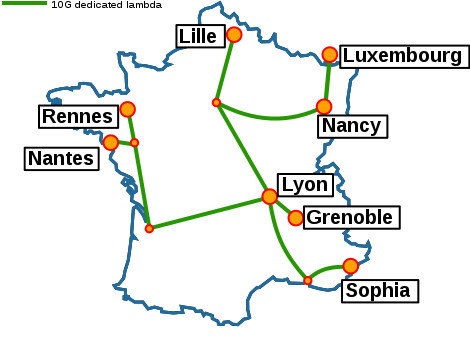
\includegraphics[scale=0.42]{figures/Renater5-g5k}
  \end{column}
\end{columns}
\end{frame}

\begin{frame}
\frametitle{Grid'5000 today (2016/11)}
\begin{center}
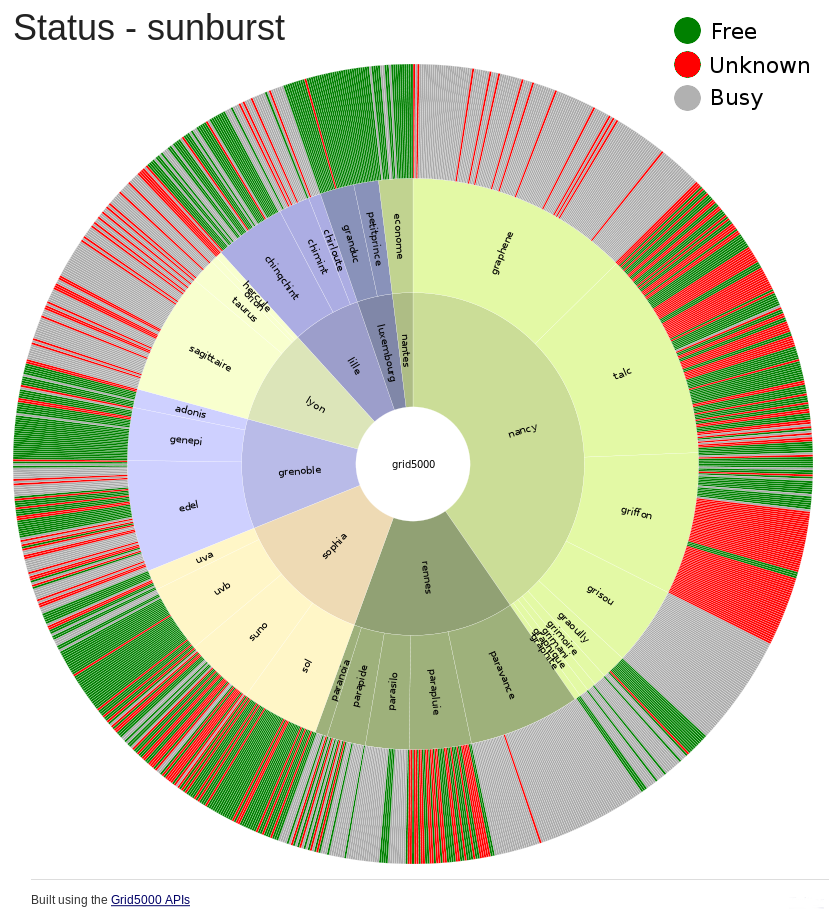
\includegraphics[scale=0.19]{figures/sunburst}
\end{center}
\end{frame}

\section{Support}
\subsection{Monitoring services and alerts}
\begin{frame}
\frametitle{Nagios dashboard}
\begin{center}
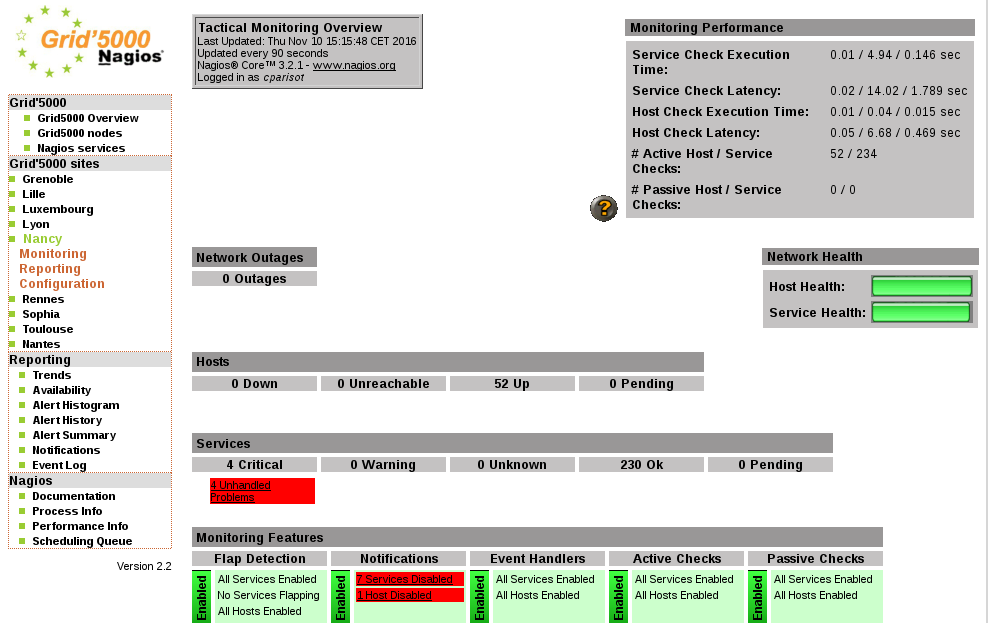
\includegraphics[scale=0.29]{figures/nagios}
\end{center}
\end{frame}

\begin{frame}
\frametitle{Nagios overview}
\begin{itemize}
\item Monitoring of the infrastructure
\item Alerts on load, ping, Hard disk failure, ...
\item One server per site
\item Reporting by mail 
\item Unified dashboard for global view
\end{itemize}
\end{frame}

\begin{frame}
\frametitle{Icinga dashboard}
\begin{center}
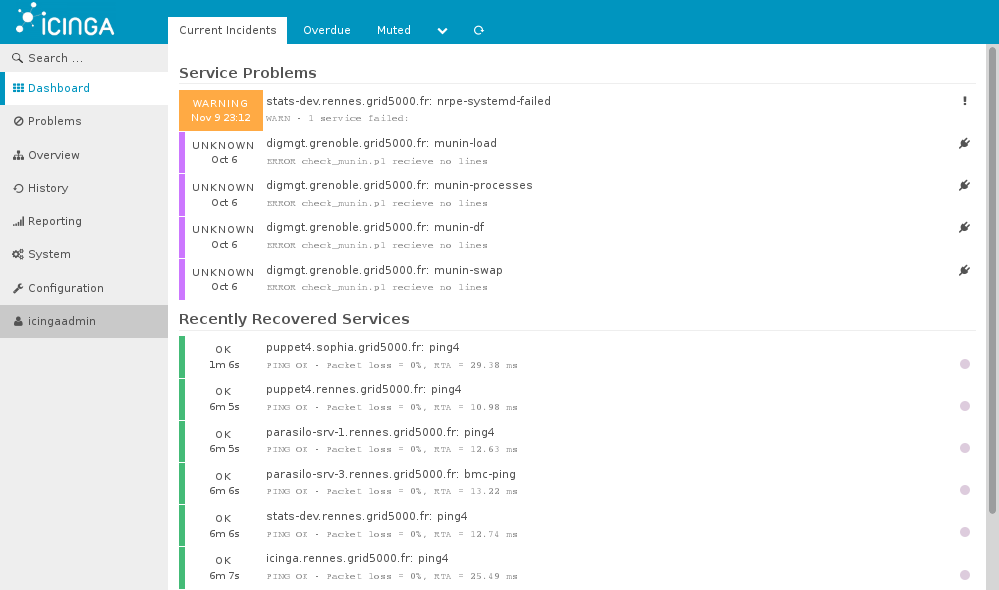
\includegraphics[scale=0.30]{figures/icinga}
\end{center}
\end{frame}

\begin{frame}
\frametitle{Icinga overview}
\begin{itemize}
\item Better UI
\item Compatibility with Nagios checks
\item Distributed monitoring
\end{itemize}
\end{frame}

\subsection{Incident and ticket}
\begin{frame}
\frametitle{Bugzilla}
\end{frame}

\section{Services orchestration}
\subsection{Xen/Puppet4}
\begin{frame}
\frametitle{Virtualisation of services infrastructure with Xen}
\end{frame}

\begin{frame}
\frametitle{Puppet for services management}
\end{frame}

\section{Example: Mediawiki upgrade}
\subsection{Package creation}
\begin{frame}
\frametitle{Create a Debian package for mediawiki}
\end{frame}

\subsection{Vagrant}
\begin{frame}
\frametitle{Vagrant as a testing environment}
\end{frame}

\subsection{Upgrade in production}
\begin{frame}
\frametitle{Tests in production}
\end{frame}

\section{Conclusion}
\begin{frame}
\frametitle{Conclusion}
:)
\end{frame}

\section*{}
\begin{frame}
\frametitle{Sources}

\end{frame}
\end{document}
